%%% Realisering af PWM controller %%%

\subsection{PWM-controller}
I det følgende afsnit testes implementeringen af PWM-controlleren. Her måles frekvensen af savtandspændingen og selve switch-frekvensen, samt signalet over current-sense modstanden både før og efter filteret.

\subsubsection{Switch-frekvens}
Først måles frekvensen af savtandspændingen. Denne frekvens måles til $160k\hertz$, hvor der ønskes $200k\hertz$. Da switch-frekvensen af indflydelse på mange ting i converteren, ændres modstanden således der opnås en frekvens på ca. $200k\hertz$. Der vælges en modstand på $33.2k\ohm$. På figur~\ref{fig:Savtand} og \ref{fig:Udgang_PWM} ses henholdsvis målingen af savtandspændingen og udgangen af PWM-controlleren. Her ses det, at der er opnået en frekvens for savtandspændingen på $192k\hertz$, og en frekvens for udgangssignalet på $102.6k\hertz$. Med et udgangspunkt på $100k\hertz$, godtages denne afvigelse. Resultaterne for analyse, simulering og realisering indføres i tabel~\ref{tab:resultat_switch_frekvens}.


\begin{table}[H] 			
	\centering
	\begin{tabularx}{\textwidth}{|X|c|c|c|}
		\hline
		\textbf{Frekvens} & \multicolumn{3}{|c|}{\textbf{Oscillator frekvens}} 										\\ \hline
		& A & S & R 									\\ \hline
		$f_{osc}$ & $200k\hertz$ & $199.6k\hertz$ & $192k\hertz$ 									\\ \hline 
		$f_s$ & $100k\hertz$ & $99.01k\hertz$ & $102.6k\hertz$ 									\\ \hline
	\end{tabularx}
	\caption{Resultater for analyse, simulering og realisering af switch-frekvens}
	\label{tab:resultat_switch_frekvens}
\end{table}


\begin{figure}[H]
	\center
	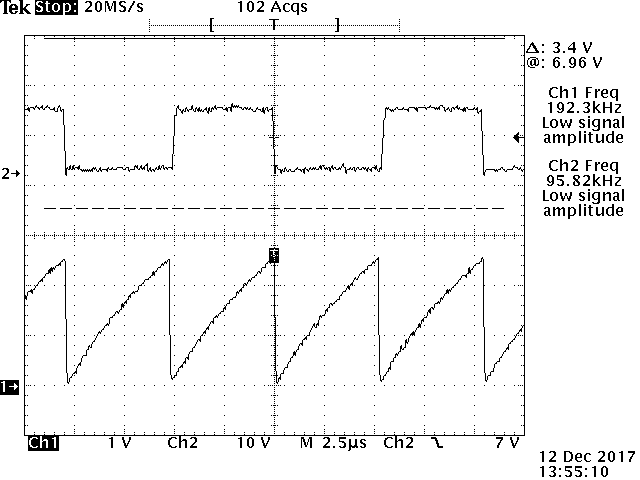
\includegraphics[max width=0.7\linewidth]{/tex/2iteration/billeder/Realisering/Savtand.png}
	\caption{Måling af savtandspænding}
	\label{fig:Savtand}
\end{figure} 

\begin{figure}[H]
	\center
	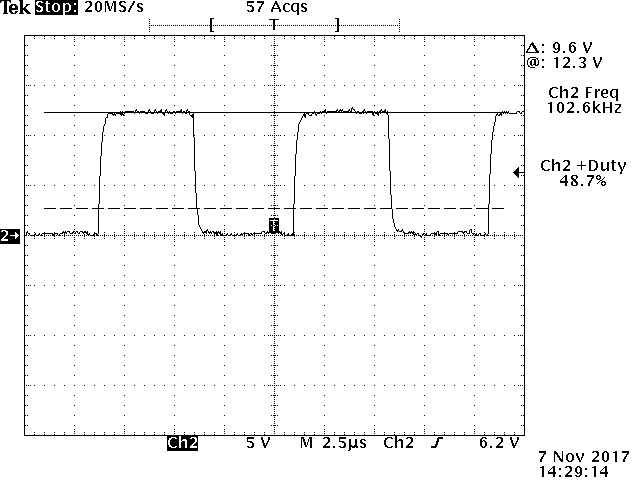
\includegraphics[max width=0.7\linewidth]{/tex/2iteration/billeder/Realisering/Udgang_PWM.png}
	\caption{Udgang af PWM-controller}
	\label{fig:Udgang_PWM}
\end{figure} 

\subsubsection{Switch-tid}
Målingen af switch-tiden er vist på figur~\ref{fig:Realisering_MOSFET_switch_tid_2}. Figuren viser MOSFET'ens drain på kannal 1, og MOSFET'ens gate på kannal 2. Her aflæses switch-tiden i MOSFET'en som længden af plateauet på gate signalet, og aflæses til ca. $120ns$. Resultaterne for analyse, simulering og realisering er indført i tabel~\ref{tab:resultat_switch_tid_2}. Her er simuleringen dog foretaget med en anden MOSFET.

\begin{table}[H] 			
	\centering
	\begin{tabularx}{\textwidth}{|X|c|c|c|}
		\hline
		\textbf{Tid} & \multicolumn{3}{|c|}{\textbf{Switch-tid}} 										\\ \hline
		& A & S & R 									\\ \hline
		$T_{ch}$ & $138.7ns$ & $103ns$ & $120ns$ 									\\ \hline 
		
	\end{tabularx}
	\caption{Resultater for analyse, simulering og realisering af switch-tid}
	\label{tab:resultat_switch_tid_2}
\end{table}

 
\begin{figure}[H]
	\center
	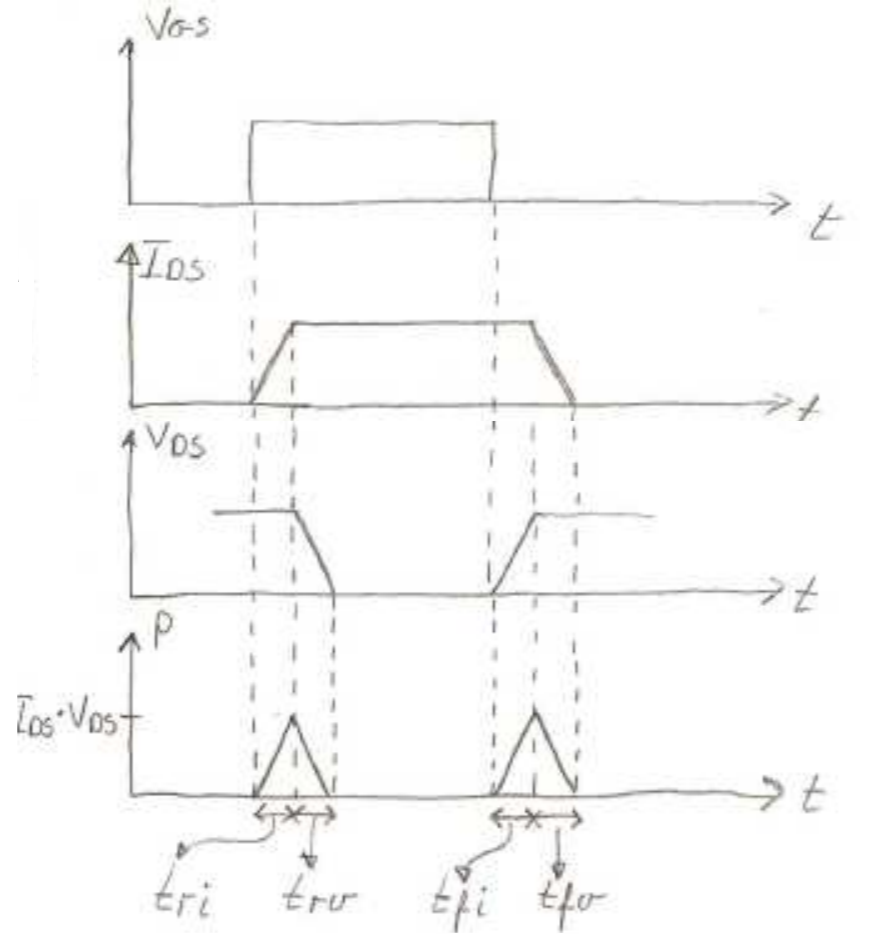
\includegraphics[max width=0.7\linewidth]{/tex/2iteration/billeder/Realisering/MOSFET_switch_tid.png}
	\caption{Switch-tid for MOSFET'en}
	\label{fig:Realisering_MOSFET_switch_tid_2}
\end{figure} 


\subsubsection{Current-sense kredsløb}
Current-sense signalet måles både før og efter filteret. Signalet før filteret ses på figur~\ref{fig:CS_U_filter}. Her ses tydeligt de spikes der ønskes filtreret, da de overstiger den egentlige peak på signalet. Figur~\ref{fig:CS_M_filter} viser signalet efter filteret. Her ses det, at de spikes der var på signalet er blevet filtreret væk. Til gengæld ses det også at signalet er blevet langsommere, ved de afrundede hjørner. Den egentlige stigetid er svær at aflæse, men det gøres den til $350ns$. Dette er ikke optimalt ved lavere duty-cycles, da det som nævnt i afsnit~\ref{CS_protection} vil påvirke systemets I/V-karakteristik. Derfor vil stige tiden af filteret blive optimeret i tredje iteration.

\noindent Resultaterne for analyse, simulering og realisering er indført i tabel~\ref{tab:resultater_cs_filter_2}.


\begin{table}[H] 			
	\centering
	\begin{tabularx}{\textwidth}{|X|c|c|c|}
		\hline
		\textbf{Tid} & \multicolumn{3}{|c|}{\textbf{Stigetid}} 										\\ \hline
		& A & S & R 									\\ \hline
		$T_{r}$ & $300ns$ & $280ns$ & $350ns$ 									\\ \hline 
		
	\end{tabularx}
	\caption{Resultater for analyse, simulering og realisering af switch-tid}
	\label{tab:resultater_cs_filter_2}
\end{table}

\begin{figure}[H]
	\center
	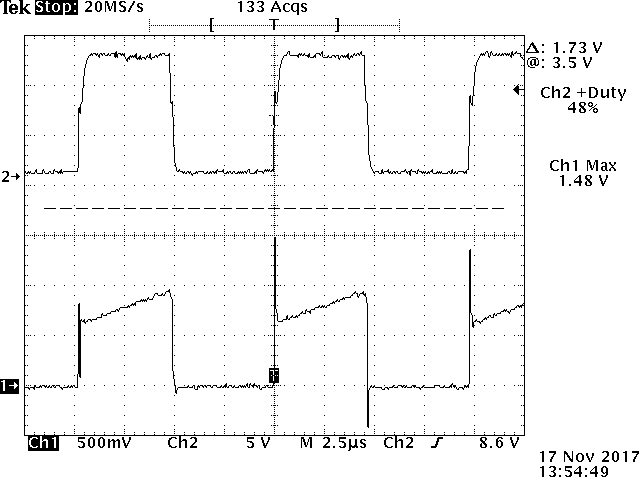
\includegraphics[max width=0.7\linewidth]{/tex/2iteration/billeder/Realisering/CS_U_filter.png}
	\caption{Current-sense signal før filter}
	\label{fig:CS_U_filter}
\end{figure}

\begin{figure}[H]
	\center
	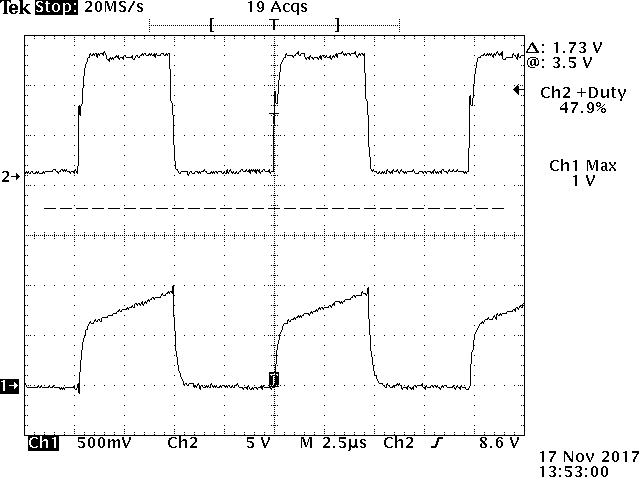
\includegraphics[max width=0.7\linewidth]{/tex/2iteration/billeder/Realisering/CS_M_filter.png}
	\caption{Current-sense signal efter filter}
	\label{fig:CS_M_filter}
\end{figure}


\subsubsection{Spændingsdeler}
Spændingsdeleren testes ved at måle indgangsspændingen til fejlforstærkeren, når udgangsspændingen er $21V$. Dette er gjort på figur~\ref{label}. Spændingen er målt til $2.5V$. Resultaterne for analyse, simulering og realisering er indført i tabel~\ref{tab:resultat_voltage_divider}.

%TODO: Skal laves, realisering mangler - Nicolai

\begin{table}[H] 			
	\centering
	\begin{tabularx}{\textwidth}{|X|c|c|c|}
		\hline
		\textbf{Spænding} & \multicolumn{3}{|c|}{\textbf{Resultater}} 		\\ \hline
		& A & S & R 									\\ \hline
		$V_{FB}$ & $2.5V$ & $2.499V$ & $??$ 									\\ \hline 
		
	\end{tabularx}
	\caption{Resultater for analyse, simulering og realisering af switch-tid}
	\label{tab:resultat_voltage_divider}
\end{table}

\subsubsection{Constant load}
Ligesom ved simuleringsafsnittet ~\ref{constant} ses der på spænding på både udgang og begge sider af transformatoren. Der er brugt en indgangsspænding på 26V og en load på $8.4\ohm$. 
Først er scoopets proper sat henover udgangen og resultatet af dette se på figur~\ref{fig: Out26V}
\begin{figure}[H]
	\center
	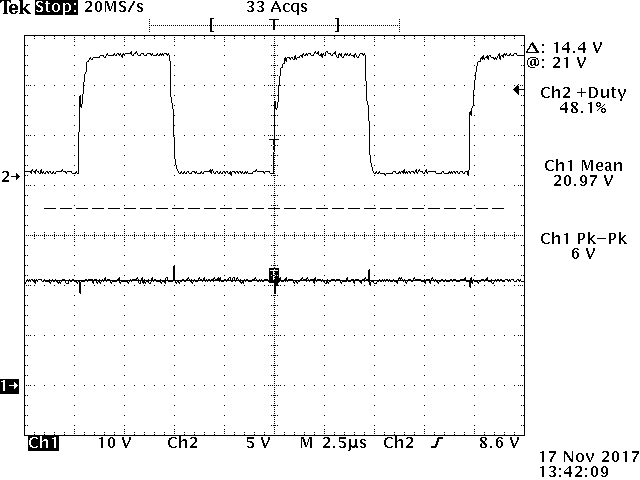
\includegraphics[max width=0.7\linewidth]{/tex/2iteration/billeder/Realisering/Output_filtreret_26V.png}
	\caption{Spændingsoutput ved 26V}
	\label{fig: Out26V}
\end{figure}
Det ses at spændingen ligger på 20.97V, altså de forventede 21V. Der kan dog identificeres nogle ret store spikes. På figur~\ref{fig: Out26Vzoom} er der zoomet ind på disse.
\begin{figure}[H]
	\center
	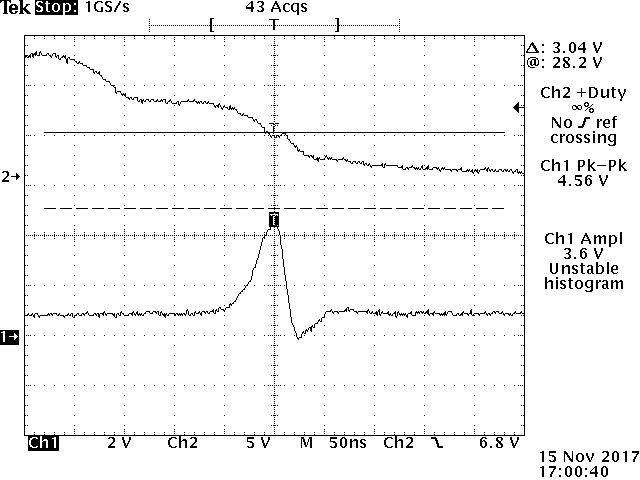
\includegraphics[max width=0.7\linewidth]{/tex/2iteration/billeder/Realisering/Outputspike_zoom.png}
	\caption{Zoomet på outputspike}
	\label{fig: Out26Vzoom}
\end{figure}
Her ses det, at spiken når helt op på en peak af 4,5V. Disse peaks skyldes switching transienter og ved figur~\ref{fig: Out26V} kan det også ses, at det sker hver gang transistoren går on eller off.

Disse transienter er endnu tydeligere ved transformatorens primær- og sekundærvikling. Først ses på figur~\ref{fig: privolt} spændingen ved den primærevikling. Det svarer til spændingen over drain på MOSFET'en. 
\begin{figure}[H]
	\center
	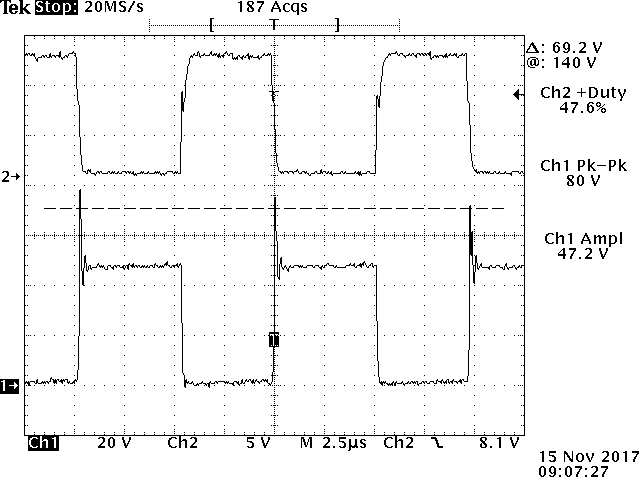
\includegraphics[max width=0.7\linewidth]{/tex/2iteration/billeder/Realisering/Transformator_Primar.png}
	\caption{Primær spænding}
	\label{fig: privolt}
\end{figure}
Det ses, at spændingen stiger med et stort peak på 80V, når transistoren går off, og ligger sig stationært på ca. 47V og falder til 0V igen, når transistoren går on. På figur~\ref{fig: prizoom} zoomes der ind på spiken.
\begin{figure}[H]
	\center
	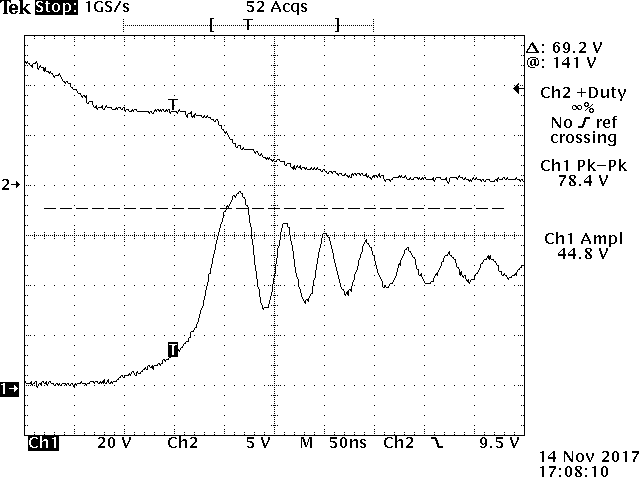
\includegraphics[max width=0.7\linewidth]{/tex/2iteration/billeder/Realisering/Transformator_Primarzoom.png}
	\caption{Zoomet på primær peak}
	\label{fig: prizoom}
\end{figure}
Udover peaken ses det, at spændingen svinger inden den ligger sig på den stationære værdi. Ses der på 2. svingningsperiode, aflæses svingningen for en periode til 40ns. Det betyder at frekvensen der ses ligger på ca:
\begin{equation} \label{svingpri}
f_{oscpri} = \frac{1}{40ns} = 25MHz
\end{equation}

På samme måde ses der på figur~\ref{fig:sek} på spændingen over den sekundære vikling. Det svarer også til spændingen på anoden af dioden. 
\begin{figure}[H]
	\center
	\includegraphics[max width=0.7\linewidth]{/tex/2iteration/billeder/Realisering/Transformator_sekundar.png}
	\caption{Sekundær spænding}
	\label{fig:sek}
\end{figure}
Her falder spændingen, når transistoren går on, og falder i første omgang med ca. 60V. Herefter ligger den på ca. 45V indtil transistoren går off og spændingen ligger sig på 20V med et mindre peak. På figur~\ref{fig:sekzoom} zoomes der ind på peaken hvor transistoren går on.
\begin{figure}[H]
	\center
	\includegraphics[max width=0.7\linewidth]{/tex/2iteration/billeder/Realisering/Transformator_sekundarzoomrise.png}
	\caption{Zoomet på sekundær peak}
	\label{fig:sekzoom}
\end{figure}
Igen observeres det, at spændingen svinger indtil den når sin stationære værdi. Her aflæses svingningen til at være 35ns, og derfor lidt kortere end ved primærviklingen. Det giver en frekvens på:
\begin{equation} \label{svingsek}
f_{oscsek} = \frac{1}{35ns} = 28.57MHz
\end{equation}

I tabellen nedenfor ses en oversigt over simulering og realisering for drain spændingen på MOSFET'en samt anoden på dioden.

\begin{table}[H] 			
	\centering
	\begin{tabularx}{\textwidth}{|X|l|l|l|l|}
		\hline
		 & \multicolumn{2}{|X|}{\textbf{Simulering}} & \multicolumn{2}{|X|}{\textbf{Realisering}} \\ \hline
		 & MOSFET & Diode & MOSFET & Diode \\ \hline
		Stationær spænding & $48V$ & $46V$ & $47V$ & $45V$ \\ \hline
		Peakspænding & $93V$ & $80V$ & $80V$ & $60V$ \\ \hline
		Svingningsfrekvens & $29.41M\hertz$ & $33.33M\hertz$ & $25.00M\hertz$ & $28.57M\hertz$ \\ \hline
	\end{tabularx}
	\caption{Simulering og realisering af spændinger over MOSFET og diode}
	\label{tab:MOSDIODE}
\end{table}

\subsubsection{Load step} \label{loadsteprea}
\noindent Load steppet er realiseret på samme måde som det blev simuleret tidligere. Med 2 $20\ohm$ modstande i parallel. Den ene med en switch, så når switchen er OFF består loaden af en $20\ohm$ modstand, men når switchen går ON er loaden $10\ohm$. Switchen blev indstillet til at sende en puls på 10ms. Oscilloskop proberne blev sat til at måle over udgangen, og resultatet af dette ses På figur~\ref{fig:belastning_samlet} 
\begin{figure}[H]
	\center
	\includegraphics[max width=0.7\linewidth]{/tex/2iteration/billeder/Realisering/belastningsamlet.png}
	\caption{Realisering af load step}
	\label{fig:belastningsamlet}
\end{figure}

Det ses hvordan spændingen falder, hvor belastningen stiger til $10\ohm$ og efter 10ms stiger spændingen, hvor belastningen igen er $20\ohm$. På figur~\ref{fig:belastning_10ohm} er der zoomet ind på dykket ved de $10\ohm$. 
\begin{figure}[H]
	\center
	\includegraphics[max width=0.7\linewidth]{/tex/2iteration/billeder/Realisering/belastningstiger(10ohm).png}
	\caption{Zoom på dyk ved 10ohm}
	\label{fig:belastning_10ohm}
\end{figure}

\noindent Det kan aflæses at spændingen når at falde med ca. $700mV$ og det tager ca. $1.5ms$ at regulere tilbage igen.

\noindent På samme måde ses stigningen ved de $20\ohm$ på figur~\ref{fig:belastning_20ohm}
\begin{figure}[H]
	\center
	\includegraphics[max width=0.7\linewidth]{/tex/2iteration/billeder/Realisering/belastningfalder(20ohm).png}
	\caption{Zoom på stigning ved 20ohm}
	\label{fig:belastning_20ohm}
\end{figure}
\noindent Her stiger spændingen med ca. $600mV$ og bruger også omkring $1.5ms$ på at regulere ind igen. 

\noindent Nedenfor ses et overblik over simuleringen af load steppet i forhold til realiseringen. 

\begin{table}[H] 			
	\centering
	\begin{tabularx}{\textwidth}{|X|l|l|l|l|}
		\hline
		& \multicolumn{2}{|l|}{\textbf{Simulering}} & \multicolumn{2}{|l|}{\textbf{Realisering}} \\ \hline
		\textbf{Belastning} & $10\ohm$ & $20\ohm$ & $10\ohm$ & $20\ohm$ \\ \hline
		Overshoot & $650mV$ & $700mV$ & $700mV$ & $600mV$  \\ \hline
		Reguleringstid & $1.6ms$ & $1.6ms$ & $1.5ms$ & $1.5ms$ \\ \hline
	\end{tabularx}
	\caption{Simulering og realisering af load step}
	\label{tab:Loadstep}
\end{table}
\noindent Det ses at simulering og realisering stemmer godt overens. Da der både ved simulering og realisering aflæses på kurver, kan usikkerheden ved det skyldes den lille afvigelse.

\subsection{Gain-fase måling} \label{gain_fase_2}
Gain-fase målingen deles op i tre, ligesom ved analysen og simuleringen. Der måles overføringsfunktion for power modulet, fejlforstærkeren, og for det samlede system. Målingerne foretages vha. en Network Analyzer af typen HP4194A. Den måler overføringsfunktionen ved at indførere et fejlsignal i tilbagekoblingen, og måle hvordan udgange ændre sig. Derved opnås åbensløjfe overføringsfunktionen. Som ved simuleringen indføres fejlsignalet over en $51.1\ohm$ modstand, placeret i serie med den første modstand i spændingsdeleren. 

Amplituden af fejlsignalet vælges til $30mV$. Ved for lille en amplitude kan signal/støj forholdet blive for småt ved lave frekvenser, mens en stor amplitude kan overstyre fejlforstærkeren. Ud fra Termas erfaringer er $30mV$ et fint udgangspunkt, men den skal muligvis justeres senere. For frekvens-sweepet vælges der et logaritmisk sweep, mens startfrekvensen vælges til $10\hertz$, og slutfrekvensen vælges til $100k\hertz$. 

Først måles gain-fasen for selve power modulet. Det gøres ved at måle mellem udgangen fra fejlforstærkeren, og udgangen fra converteren. Det er vist på figur~\ref{fig:realisering_gain_fase_power}. Der vist bode plot for både analyse og realisering. På grund af usikkerhed i simuleringen er denne del udeladt. Gain for realiseringen er den blå, mens gain for analysen er den grønne stiplede. Fasen for realiseringen er er den røde, mens fasen for analysen er den stiplede lilla. Det ses at gain-fase karakteristikken ser ud som forventet ud fra analysen. Det er først ved de høje frekvenser målingen afviger fra analysen. Båndbredden for power modulet aflæses til ca. $1400\hertz$, mens DC-gain aflæses til ca. $20.3\decibel$.

\begin{figure}[H]
	\center
	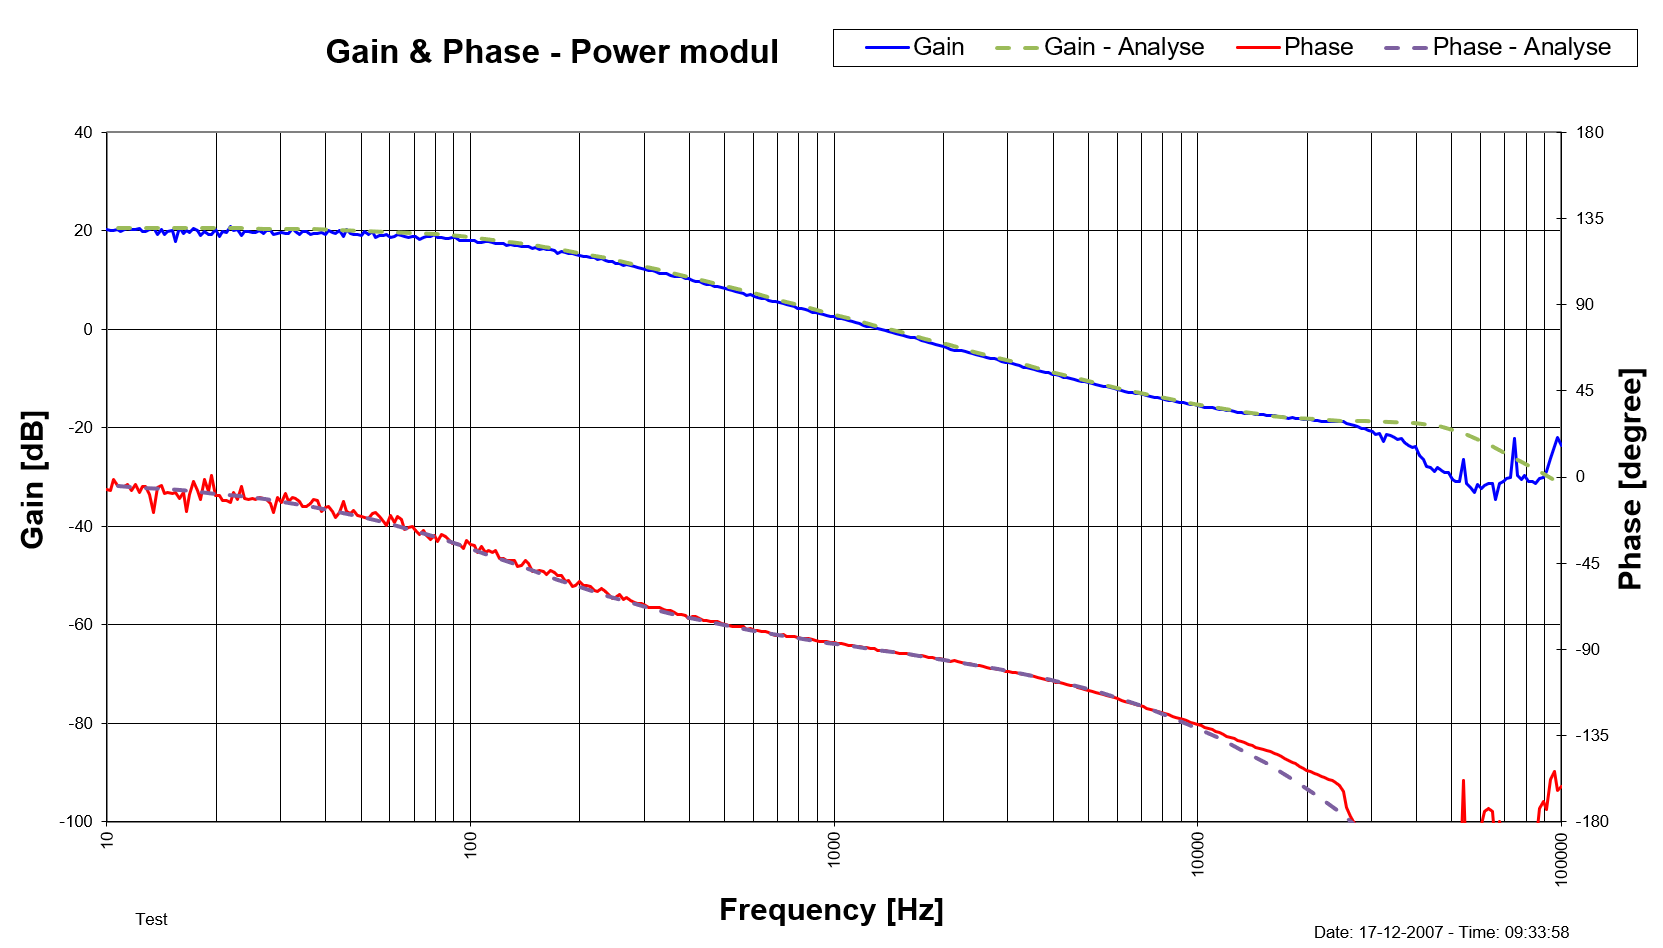
\includegraphics[max width=0.7\linewidth]{/tex/2iteration/billeder/Realisering/Realisering_gain_fase_power.png}
	\caption{Realisering af gain-fase for power modul}
	\label{fig:realisering_gain_fase_power}
\end{figure}

%TODO: Beskriv fejlforstærker når målinger hentes ved Terma


Til sidst måles den samlede overføringsfunktion for systemet. Her måles der over den modstand, hvor fejlsignalet indføres. Det svarer til at måle fra indgangen af fejlforstærkeren til udgangen af converteren. Bode plottet for både analyse og realiseringen er vist på figur~\ref{fig:realisering_gain_fase_tot}. Gain for realiseringen er den blå, mens gain for analysen er den grønne stiplede. Fasen for realiseringen er er den røde, mens fasen for analysen er den stiplede lilla. På bode plottet ses det at der er en smule større afvigelse, både ved gain og fasen. På trods af afvigelsen aflæses båndbredden dog nogenlunde til det samme på ca. $900\hertz$. Fase-margin aflæses til ca. $62^\circ$, og gain-margin aflæses til ca. $24\decibel$. Holdt op mod analysen var det forventet at opnå en fase-margin på $74.3^\circ$ og en gain-margin på $24\decibel$. Afvigelsen i fase-margin ses på figur~\ref{fig:realisering_gain_fase_tot}, da den faktiske fase ligger under den analyserede. 

\begin{figure}[H]
	\center
	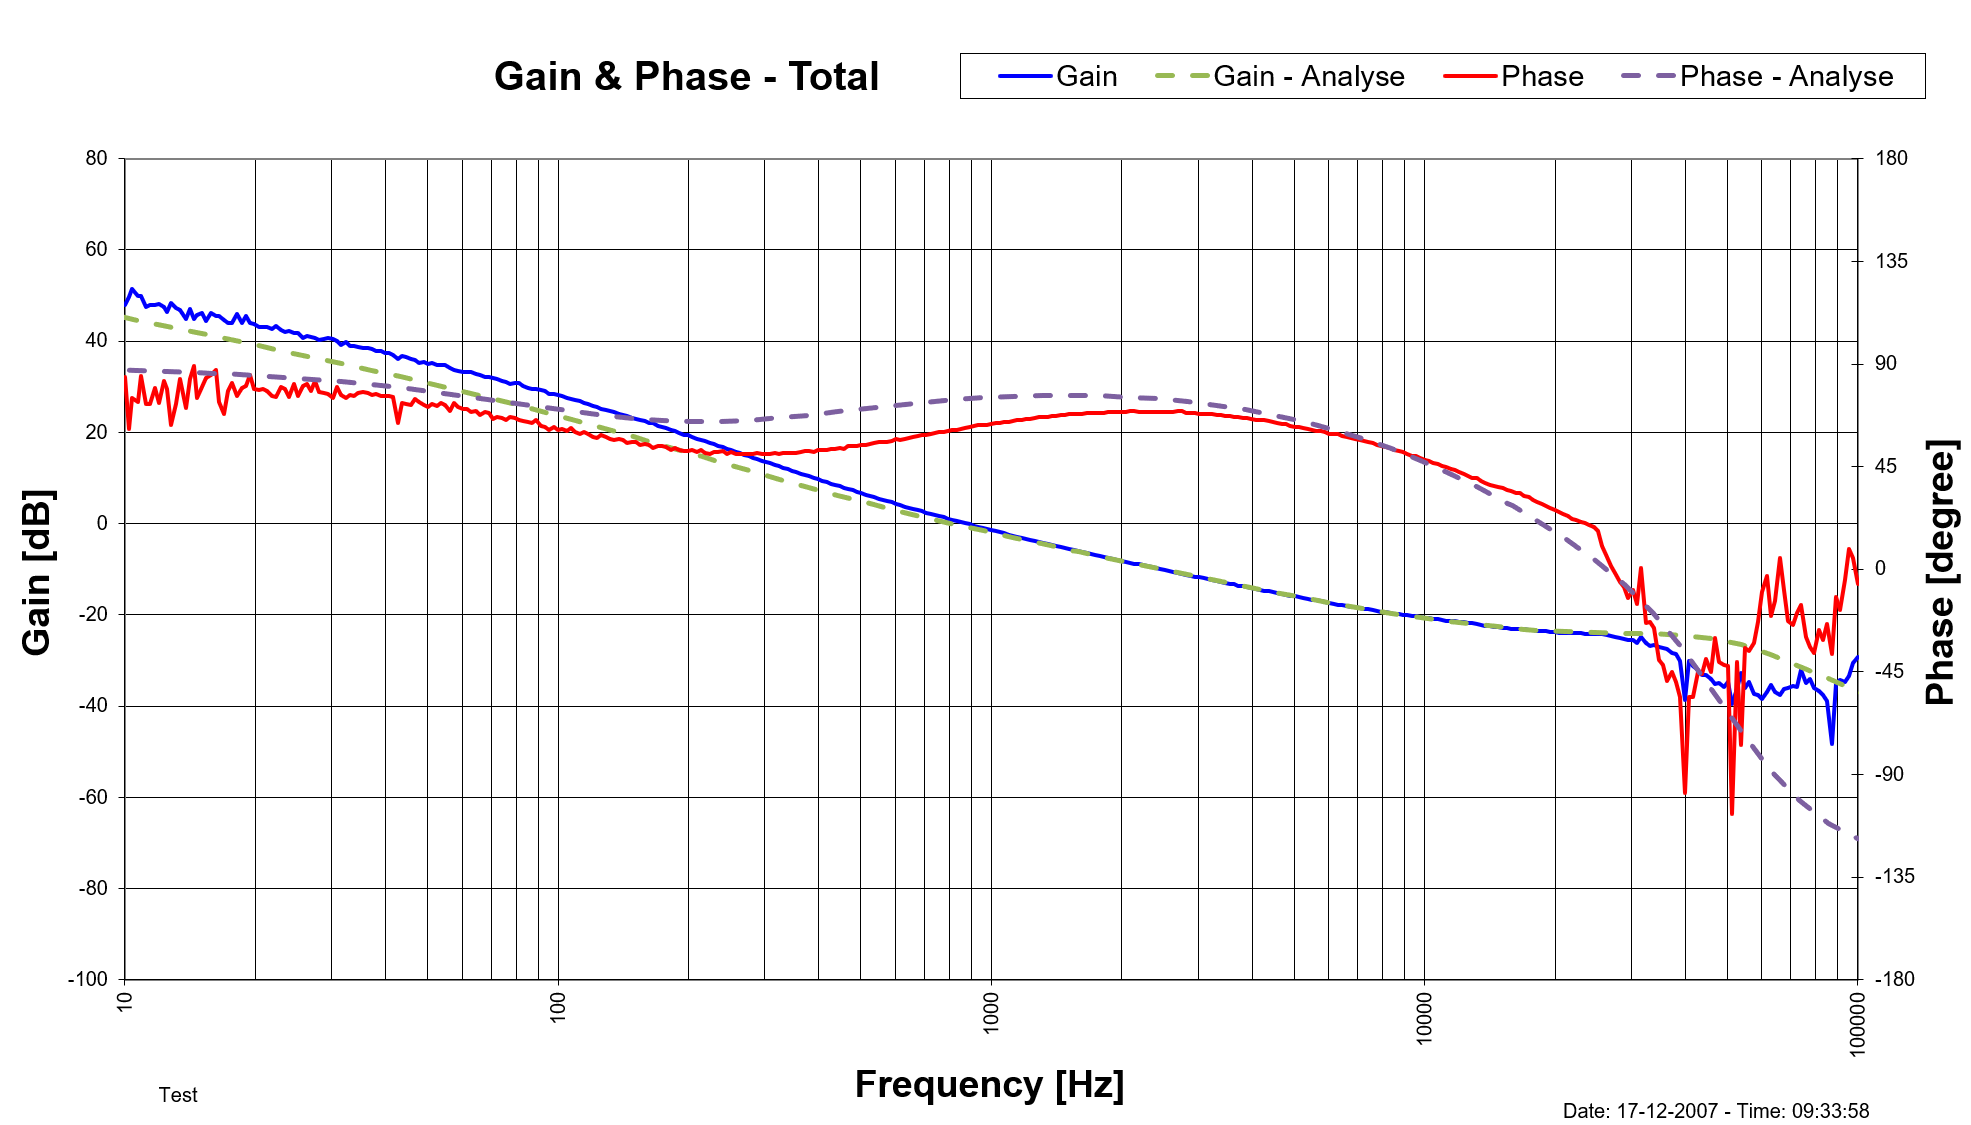
\includegraphics[max width=0.7\linewidth]{/tex/2iteration/billeder/Realisering/Realisering_gain_fase_tot.png}
	\caption{Realisering af gain-fase for hele systemet}
	\label{fig:realisering_gain_fase_tot}
\end{figure}
















